\section{stats.h File Reference}
\label{zesto_2stats_8h}\index{stats.h@{stats.h}}
{\tt \#include $<$stdio.h$>$}\par
{\tt \#include \char`\"{}host.h\char`\"{}}\par
{\tt \#include \char`\"{}machine.h\char`\"{}}\par
{\tt \#include \char`\"{}eval.h\char`\"{}}\par


Include dependency graph for zesto/stats.h:\nopagebreak
\begin{figure}[H]
\begin{center}
\leavevmode
\includegraphics[width=412pt]{zesto_2stats_8h__incl}
\end{center}
\end{figure}


This graph shows which files directly or indirectly include this file:\nopagebreak
\begin{figure}[H]
\begin{center}
\leavevmode
\includegraphics[width=420pt]{zesto_2stats_8h__dep__incl}
\end{center}
\end{figure}
\subsection*{Classes}
\begin{CompactItemize}
\item 
struct {\bf bucket\_\-t}
\item 
struct {\bf stat\_\-stat\_\-t}
\item 
union {\bf stat\_\-stat\_\-t::stat\_\-stat\_\-t::stat\_\-variant\_\-t}
\item 
struct {\bf stat\_\-stat\_\-t::stat\_\-stat\_\-t::stat\_\-variant\_\-t::stat\_\-stat\_\-t::stat\_\-variant\_\-t::stat\_\-for\_\-int\_\-t}
\item 
struct {\bf stat\_\-stat\_\-t::stat\_\-stat\_\-t::stat\_\-variant\_\-t::stat\_\-stat\_\-t::stat\_\-variant\_\-t::stat\_\-for\_\-uint\_\-t}
\item 
struct {\bf stat\_\-stat\_\-t::stat\_\-stat\_\-t::stat\_\-variant\_\-t::stat\_\-stat\_\-t::stat\_\-variant\_\-t::stat\_\-for\_\-qword\_\-t}
\item 
struct {\bf stat\_\-stat\_\-t::stat\_\-stat\_\-t::stat\_\-variant\_\-t::stat\_\-stat\_\-t::stat\_\-variant\_\-t::stat\_\-for\_\-sqword\_\-t}
\item 
struct {\bf stat\_\-stat\_\-t::stat\_\-stat\_\-t::stat\_\-variant\_\-t::stat\_\-stat\_\-t::stat\_\-variant\_\-t::stat\_\-for\_\-float\_\-t}
\item 
struct {\bf stat\_\-stat\_\-t::stat\_\-stat\_\-t::stat\_\-variant\_\-t::stat\_\-stat\_\-t::stat\_\-variant\_\-t::stat\_\-for\_\-double\_\-t}
\item 
struct {\bf stat\_\-stat\_\-t::stat\_\-stat\_\-t::stat\_\-variant\_\-t::stat\_\-stat\_\-t::stat\_\-variant\_\-t::stat\_\-for\_\-dist\_\-t}
\item 
struct {\bf stat\_\-stat\_\-t::stat\_\-stat\_\-t::stat\_\-variant\_\-t::stat\_\-stat\_\-t::stat\_\-variant\_\-t::stat\_\-for\_\-sdist\_\-t}
\item 
struct {\bf stat\_\-stat\_\-t::stat\_\-stat\_\-t::stat\_\-variant\_\-t::stat\_\-stat\_\-t::stat\_\-variant\_\-t::stat\_\-for\_\-formula\_\-t}
\item 
struct {\bf stat\_\-stat\_\-t::stat\_\-stat\_\-t::stat\_\-variant\_\-t::stat\_\-stat\_\-t::stat\_\-variant\_\-t::stat\_\-for\_\-string\_\-t}
\item 
struct {\bf stat\_\-stat\_\-t::stat\_\-stat\_\-t::stat\_\-variant\_\-t::stat\_\-stat\_\-t::stat\_\-variant\_\-t::stat\_\-for\_\-note\_\-t}
\item 
struct {\bf stat\_\-sdb\_\-t}
\end{CompactItemize}
\subsection*{Defines}
\begin{CompactItemize}
\item 
\#define {\bf HTAB\_\-SZ}~1024
\item 
\#define {\bf HTAB\_\-HASH}(I)~((((I) $>$$>$ 8) $^\wedge$ (I)) \& (HTAB\_\-SZ - 1))
\item 
\#define {\bf PF\_\-COUNT}~0x0001
\item 
\#define {\bf PF\_\-PDF}~0x0002
\item 
\#define {\bf PF\_\-CDF}~0x0004
\item 
\#define {\bf PF\_\-ALL}~(PF\_\-COUNT$|$PF\_\-PDF$|$PF\_\-CDF)
\end{CompactItemize}
\subsection*{Typedefs}
\begin{CompactItemize}
\item 
typedef void($\ast$ {\bf print\_\-fn\_\-t} )(struct {\bf stat\_\-stat\_\-t} $\ast$stat, {\bf md\_\-addr\_\-t} index, int count, double sum, double total)
\end{CompactItemize}
\subsection*{Enumerations}
\begin{CompactItemize}
\item 
enum {\bf stat\_\-class\_\-t} \{ \par
{\bf sc\_\-int} =  0, 
{\bf sc\_\-uint}, 
{\bf sc\_\-qword}, 
{\bf sc\_\-sqword}, 
\par
{\bf sc\_\-float}, 
{\bf sc\_\-double}, 
{\bf sc\_\-dist}, 
{\bf sc\_\-sdist}, 
\par
{\bf sc\_\-formula}, 
{\bf sc\_\-string}, 
{\bf sc\_\-note}, 
{\bf sc\_\-NUM}
 \}
\end{CompactItemize}
\subsection*{Functions}
\begin{CompactItemize}
\item 
struct {\bf eval\_\-value\_\-t} {\bf stat\_\-eval\_\-ident} (struct {\bf eval\_\-state\_\-t} $\ast$es)
\item 
struct {\bf stat\_\-sdb\_\-t} $\ast$ {\bf stat\_\-new} (void)
\item 
void {\bf stat\_\-delete} (struct {\bf stat\_\-sdb\_\-t} $\ast$sdb)
\item 
struct {\bf stat\_\-stat\_\-t} $\ast$ {\bf stat\_\-reg\_\-int} (struct {\bf stat\_\-sdb\_\-t} $\ast$sdb, int print\_\-me, const char $\ast$name, const char $\ast$desc, int $\ast$var, int init\_\-val, const char $\ast$format)
\item 
struct {\bf stat\_\-stat\_\-t} $\ast$ {\bf stat\_\-reg\_\-uint} (struct {\bf stat\_\-sdb\_\-t} $\ast$sdb, int print\_\-me, const char $\ast$name, const char $\ast$desc, unsigned int $\ast$var, unsigned int init\_\-val, const char $\ast$format)
\item 
struct {\bf stat\_\-stat\_\-t} $\ast$ {\bf stat\_\-reg\_\-qword} (struct {\bf stat\_\-sdb\_\-t} $\ast$sdb, int print\_\-me, const char $\ast$name, const char $\ast$desc, qword\_\-t $\ast$var, qword\_\-t init\_\-val, const char $\ast$format)
\item 
struct {\bf stat\_\-stat\_\-t} $\ast$ {\bf stat\_\-reg\_\-sqword} (struct {\bf stat\_\-sdb\_\-t} $\ast$sdb, int print\_\-me, const char $\ast$name, const char $\ast$desc, sqword\_\-t $\ast$var, sqword\_\-t init\_\-val, const char $\ast$format)
\item 
struct {\bf stat\_\-stat\_\-t} $\ast$ {\bf stat\_\-reg\_\-float} (struct {\bf stat\_\-sdb\_\-t} $\ast$sdb, int print\_\-me, const char $\ast$name, const char $\ast$desc, float $\ast$var, float init\_\-val, const char $\ast$format)
\item 
struct {\bf stat\_\-stat\_\-t} $\ast$ {\bf stat\_\-reg\_\-double} (struct {\bf stat\_\-sdb\_\-t} $\ast$sdb, int print\_\-me, const char $\ast$name, const char $\ast$desc, double $\ast$var, double init\_\-val, const char $\ast$format)
\item 
struct {\bf stat\_\-stat\_\-t} $\ast$ {\bf stat\_\-reg\_\-dist} (struct {\bf stat\_\-sdb\_\-t} $\ast$sdb, const char $\ast$name, const char $\ast$desc, unsigned int init\_\-val, unsigned int arr\_\-sz, unsigned int bucket\_\-sz, int pf, const char $\ast$format, const char $\ast$$\ast$imap, {\bf print\_\-fn\_\-t} print\_\-fn)
\item 
struct {\bf stat\_\-stat\_\-t} $\ast$ {\bf stat\_\-reg\_\-sdist} (struct {\bf stat\_\-sdb\_\-t} $\ast$sdb, const char $\ast$name, const char $\ast$desc, unsigned int init\_\-val, int pf, const char $\ast$format, {\bf print\_\-fn\_\-t} print\_\-fn)
\item 
void {\bf stat\_\-add\_\-samples} (struct {\bf stat\_\-stat\_\-t} $\ast$stat, {\bf md\_\-addr\_\-t} index, int nsamples)
\item 
void {\bf stat\_\-add\_\-sample} (struct {\bf stat\_\-stat\_\-t} $\ast$stat, {\bf md\_\-addr\_\-t} index)
\item 
struct {\bf stat\_\-stat\_\-t} $\ast$ {\bf stat\_\-reg\_\-formula} (struct {\bf stat\_\-sdb\_\-t} $\ast$sdb, int print\_\-me, const char $\ast$name, const char $\ast$desc, const char $\ast$formula, const char $\ast$format)
\item 
struct {\bf stat\_\-stat\_\-t} $\ast$ {\bf stat\_\-reg\_\-string} (struct {\bf stat\_\-sdb\_\-t} $\ast$sdb, const char $\ast$name, const char $\ast$desc, const char $\ast$var, const char $\ast$format)
\item 
struct {\bf stat\_\-stat\_\-t} $\ast$ {\bf stat\_\-reg\_\-note} (struct {\bf stat\_\-sdb\_\-t} $\ast$sdb, const char $\ast$note)
\item 
void {\bf stat\_\-print\_\-stat} (struct {\bf stat\_\-sdb\_\-t} $\ast$sdb, struct {\bf stat\_\-stat\_\-t} $\ast$stat, FILE $\ast$fd)
\item 
void {\bf stat\_\-print\_\-stats} (struct {\bf stat\_\-sdb\_\-t} $\ast$sdb, FILE $\ast$fd)
\item 
struct {\bf stat\_\-stat\_\-t} $\ast$ {\bf stat\_\-find\_\-stat} (struct {\bf stat\_\-sdb\_\-t} $\ast$sdb, const char $\ast$stat\_\-name)
\item 
void {\bf print\_\-sdist} (struct {\bf stat\_\-stat\_\-t} $\ast$stat, FILE $\ast$fd)
\item 
void {\bf print\_\-dist} (struct {\bf stat\_\-stat\_\-t} $\ast$stat, FILE $\ast$fd)
\end{CompactItemize}


\subsection{Define Documentation}
\index{zesto/stats.h@{zesto/stats.h}!HTAB\_\-HASH@{HTAB\_\-HASH}}
\index{HTAB\_\-HASH@{HTAB\_\-HASH}!zesto/stats.h@{zesto/stats.h}}
\subsubsection[{HTAB\_\-HASH}]{\setlength{\rightskip}{0pt plus 5cm}\#define HTAB\_\-HASH(I)~((((I) $>$$>$ 8) $^\wedge$ (I)) \& (HTAB\_\-SZ - 1))}\label{zesto_2stats_8h_cd35c0c70acba6ef53e0e20c15f09395}




Definition at line 93 of file zesto/stats.h.\index{zesto/stats.h@{zesto/stats.h}!HTAB\_\-SZ@{HTAB\_\-SZ}}
\index{HTAB\_\-SZ@{HTAB\_\-SZ}!zesto/stats.h@{zesto/stats.h}}
\subsubsection[{HTAB\_\-SZ}]{\setlength{\rightskip}{0pt plus 5cm}\#define HTAB\_\-SZ~1024}\label{zesto_2stats_8h_a9de58549ac3f9cc4c23ce618b91b53f}




Definition at line 92 of file zesto/stats.h.\index{zesto/stats.h@{zesto/stats.h}!PF\_\-ALL@{PF\_\-ALL}}
\index{PF\_\-ALL@{PF\_\-ALL}!zesto/stats.h@{zesto/stats.h}}
\subsubsection[{PF\_\-ALL}]{\setlength{\rightskip}{0pt plus 5cm}\#define PF\_\-ALL~(PF\_\-COUNT$|$PF\_\-PDF$|$PF\_\-CDF)}\label{zesto_2stats_8h_3ea4fdaa5e25d50a550571bb829f709c}




Definition at line 109 of file zesto/stats.h.\index{zesto/stats.h@{zesto/stats.h}!PF\_\-CDF@{PF\_\-CDF}}
\index{PF\_\-CDF@{PF\_\-CDF}!zesto/stats.h@{zesto/stats.h}}
\subsubsection[{PF\_\-CDF}]{\setlength{\rightskip}{0pt plus 5cm}\#define PF\_\-CDF~0x0004}\label{zesto_2stats_8h_0cf410069cb11a44448cea46cf11c047}




Definition at line 108 of file zesto/stats.h.\index{zesto/stats.h@{zesto/stats.h}!PF\_\-COUNT@{PF\_\-COUNT}}
\index{PF\_\-COUNT@{PF\_\-COUNT}!zesto/stats.h@{zesto/stats.h}}
\subsubsection[{PF\_\-COUNT}]{\setlength{\rightskip}{0pt plus 5cm}\#define PF\_\-COUNT~0x0001}\label{zesto_2stats_8h_a2ea8c2ebd4b70b8bb60561c6fada674}




Definition at line 106 of file zesto/stats.h.

Referenced by core\_\-fetch\_\-STM\_\-t::reg\_\-stats(), core\_\-fetch\_\-DPM\_\-t::reg\_\-stats(), core\_\-decode\_\-STM\_\-t::reg\_\-stats(), core\_\-decode\_\-DPM\_\-t::reg\_\-stats(), core\_\-commit\_\-STM\_\-t::reg\_\-stats(), core\_\-commit\_\-DPM\_\-t::reg\_\-stats(), core\_\-alloc\_\-STM\_\-t::reg\_\-stats(), and core\_\-alloc\_\-DPM\_\-t::reg\_\-stats().\index{zesto/stats.h@{zesto/stats.h}!PF\_\-PDF@{PF\_\-PDF}}
\index{PF\_\-PDF@{PF\_\-PDF}!zesto/stats.h@{zesto/stats.h}}
\subsubsection[{PF\_\-PDF}]{\setlength{\rightskip}{0pt plus 5cm}\#define PF\_\-PDF~0x0002}\label{zesto_2stats_8h_7e857abbfb7e3dc6d4446052a96653a3}




Definition at line 107 of file zesto/stats.h.

Referenced by core\_\-fetch\_\-STM\_\-t::reg\_\-stats(), core\_\-fetch\_\-DPM\_\-t::reg\_\-stats(), core\_\-decode\_\-STM\_\-t::reg\_\-stats(), core\_\-decode\_\-DPM\_\-t::reg\_\-stats(), core\_\-commit\_\-STM\_\-t::reg\_\-stats(), core\_\-commit\_\-DPM\_\-t::reg\_\-stats(), core\_\-alloc\_\-STM\_\-t::reg\_\-stats(), and core\_\-alloc\_\-DPM\_\-t::reg\_\-stats().

\subsection{Typedef Documentation}
\index{zesto/stats.h@{zesto/stats.h}!print\_\-fn\_\-t@{print\_\-fn\_\-t}}
\index{print\_\-fn\_\-t@{print\_\-fn\_\-t}!zesto/stats.h@{zesto/stats.h}}
\subsubsection[{print\_\-fn\_\-t}]{\setlength{\rightskip}{0pt plus 5cm}typedef void($\ast$ {\bf print\_\-fn\_\-t})(struct {\bf stat\_\-stat\_\-t} $\ast$stat,{\bf md\_\-addr\_\-t} index,int count,double sum,double total)}\label{zesto_2stats_8h_e4b17f8ba8e81941519f3e55dd08a4ff}




Definition at line 115 of file zesto/stats.h.

\subsection{Enumeration Type Documentation}
\index{zesto/stats.h@{zesto/stats.h}!stat\_\-class\_\-t@{stat\_\-class\_\-t}}
\index{stat\_\-class\_\-t@{stat\_\-class\_\-t}!zesto/stats.h@{zesto/stats.h}}
\subsubsection[{stat\_\-class\_\-t}]{\setlength{\rightskip}{0pt plus 5cm}enum {\bf stat\_\-class\_\-t}}\label{zesto_2stats_8h_7caa50c971612efca8f45cbf1106e596}


\begin{Desc}
\item[Enumerator: ]\par
\begin{description}
\index{sc\_\-int@{sc\_\-int}!zesto/stats.h@{zesto/stats.h}}\index{zesto/stats.h@{zesto/stats.h}!sc\_\-int@{sc\_\-int}}\item[{\em 
sc\_\-int\label{zesto_2stats_8h_7caa50c971612efca8f45cbf1106e5962bd59ac0b21ec35ef900837744b7e2f6}
}]\index{sc\_\-uint@{sc\_\-uint}!zesto/stats.h@{zesto/stats.h}}\index{zesto/stats.h@{zesto/stats.h}!sc\_\-uint@{sc\_\-uint}}\item[{\em 
sc\_\-uint\label{zesto_2stats_8h_7caa50c971612efca8f45cbf1106e596990da3af9bb5feeda3bd4b1ab35065f0}
}]\index{sc\_\-qword@{sc\_\-qword}!zesto/stats.h@{zesto/stats.h}}\index{zesto/stats.h@{zesto/stats.h}!sc\_\-qword@{sc\_\-qword}}\item[{\em 
sc\_\-qword\label{zesto_2stats_8h_7caa50c971612efca8f45cbf1106e59643c3f672f0566de30cacd45bb5814b49}
}]\index{sc\_\-sqword@{sc\_\-sqword}!zesto/stats.h@{zesto/stats.h}}\index{zesto/stats.h@{zesto/stats.h}!sc\_\-sqword@{sc\_\-sqword}}\item[{\em 
sc\_\-sqword\label{zesto_2stats_8h_7caa50c971612efca8f45cbf1106e596e03324053fb098292f6cfc50e98f70ab}
}]\index{sc\_\-float@{sc\_\-float}!zesto/stats.h@{zesto/stats.h}}\index{zesto/stats.h@{zesto/stats.h}!sc\_\-float@{sc\_\-float}}\item[{\em 
sc\_\-float\label{zesto_2stats_8h_7caa50c971612efca8f45cbf1106e596ca678c49a3cffb48af18908c36a28856}
}]\index{sc\_\-double@{sc\_\-double}!zesto/stats.h@{zesto/stats.h}}\index{zesto/stats.h@{zesto/stats.h}!sc\_\-double@{sc\_\-double}}\item[{\em 
sc\_\-double\label{zesto_2stats_8h_7caa50c971612efca8f45cbf1106e5964bdab5b3d74294acfd84efa21ca97d01}
}]\index{sc\_\-dist@{sc\_\-dist}!zesto/stats.h@{zesto/stats.h}}\index{zesto/stats.h@{zesto/stats.h}!sc\_\-dist@{sc\_\-dist}}\item[{\em 
sc\_\-dist\label{zesto_2stats_8h_7caa50c971612efca8f45cbf1106e59678bd6bf930700d807a586026652f9558}
}]\index{sc\_\-sdist@{sc\_\-sdist}!zesto/stats.h@{zesto/stats.h}}\index{zesto/stats.h@{zesto/stats.h}!sc\_\-sdist@{sc\_\-sdist}}\item[{\em 
sc\_\-sdist\label{zesto_2stats_8h_7caa50c971612efca8f45cbf1106e596eec35818917bbdd89c0ca202d966ecdb}
}]\index{sc\_\-formula@{sc\_\-formula}!zesto/stats.h@{zesto/stats.h}}\index{zesto/stats.h@{zesto/stats.h}!sc\_\-formula@{sc\_\-formula}}\item[{\em 
sc\_\-formula\label{zesto_2stats_8h_7caa50c971612efca8f45cbf1106e596c764056d87be9592100bdbc0c729fb5f}
}]\index{sc\_\-string@{sc\_\-string}!zesto/stats.h@{zesto/stats.h}}\index{zesto/stats.h@{zesto/stats.h}!sc\_\-string@{sc\_\-string}}\item[{\em 
sc\_\-string\label{zesto_2stats_8h_7caa50c971612efca8f45cbf1106e5963347ce5c90c6634f001634d8ab4b1e7a}
}]\index{sc\_\-note@{sc\_\-note}!zesto/stats.h@{zesto/stats.h}}\index{zesto/stats.h@{zesto/stats.h}!sc\_\-note@{sc\_\-note}}\item[{\em 
sc\_\-note\label{zesto_2stats_8h_7caa50c971612efca8f45cbf1106e596805b2b994341a4b8f3a86f07b7388ea1}
}]\index{sc\_\-NUM@{sc\_\-NUM}!zesto/stats.h@{zesto/stats.h}}\index{zesto/stats.h@{zesto/stats.h}!sc\_\-NUM@{sc\_\-NUM}}\item[{\em 
sc\_\-NUM\label{zesto_2stats_8h_7caa50c971612efca8f45cbf1106e5968b6568f9e4b06cb9657df8a48956de73}
}]\end{description}
\end{Desc}



Definition at line 76 of file zesto/stats.h.

\subsection{Function Documentation}
\index{zesto/stats.h@{zesto/stats.h}!print\_\-dist@{print\_\-dist}}
\index{print\_\-dist@{print\_\-dist}!zesto/stats.h@{zesto/stats.h}}
\subsubsection[{print\_\-dist}]{\setlength{\rightskip}{0pt plus 5cm}void print\_\-dist (struct {\bf stat\_\-stat\_\-t} $\ast$ {\em stat}, \/  FILE $\ast$ {\em fd})}\label{zesto_2stats_8h_162e72b041405e38ba5550fe16b345c9}


\index{zesto/stats.h@{zesto/stats.h}!print\_\-sdist@{print\_\-sdist}}
\index{print\_\-sdist@{print\_\-sdist}!zesto/stats.h@{zesto/stats.h}}
\subsubsection[{print\_\-sdist}]{\setlength{\rightskip}{0pt plus 5cm}void print\_\-sdist (struct {\bf stat\_\-stat\_\-t} $\ast$ {\em stat}, \/  FILE $\ast$ {\em fd})}\label{zesto_2stats_8h_d6343ab164d17218e4312f17318bec2b}


\index{zesto/stats.h@{zesto/stats.h}!stat\_\-add\_\-sample@{stat\_\-add\_\-sample}}
\index{stat\_\-add\_\-sample@{stat\_\-add\_\-sample}!zesto/stats.h@{zesto/stats.h}}
\subsubsection[{stat\_\-add\_\-sample}]{\setlength{\rightskip}{0pt plus 5cm}void stat\_\-add\_\-sample (struct {\bf stat\_\-stat\_\-t} $\ast$ {\em stat}, \/  {\bf md\_\-addr\_\-t} {\em index})}\label{zesto_2stats_8h_702503b8068fdcce1dc8712be9791d42}




Referenced by core\_\-decode\_\-STM\_\-t::check\_\-flush(), core\_\-decode\_\-DPM\_\-t::check\_\-flush(), core\_\-fetch\_\-STM\_\-t::step(), core\_\-fetch\_\-DPM\_\-t::step(), core\_\-decode\_\-STM\_\-t::step(), core\_\-decode\_\-DPM\_\-t::step(), core\_\-commit\_\-STM\_\-t::step(), core\_\-commit\_\-DPM\_\-t::step(), core\_\-alloc\_\-STM\_\-t::step(), and core\_\-alloc\_\-DPM\_\-t::step().

Here is the caller graph for this function:\nopagebreak
\begin{figure}[H]
\begin{center}
\leavevmode
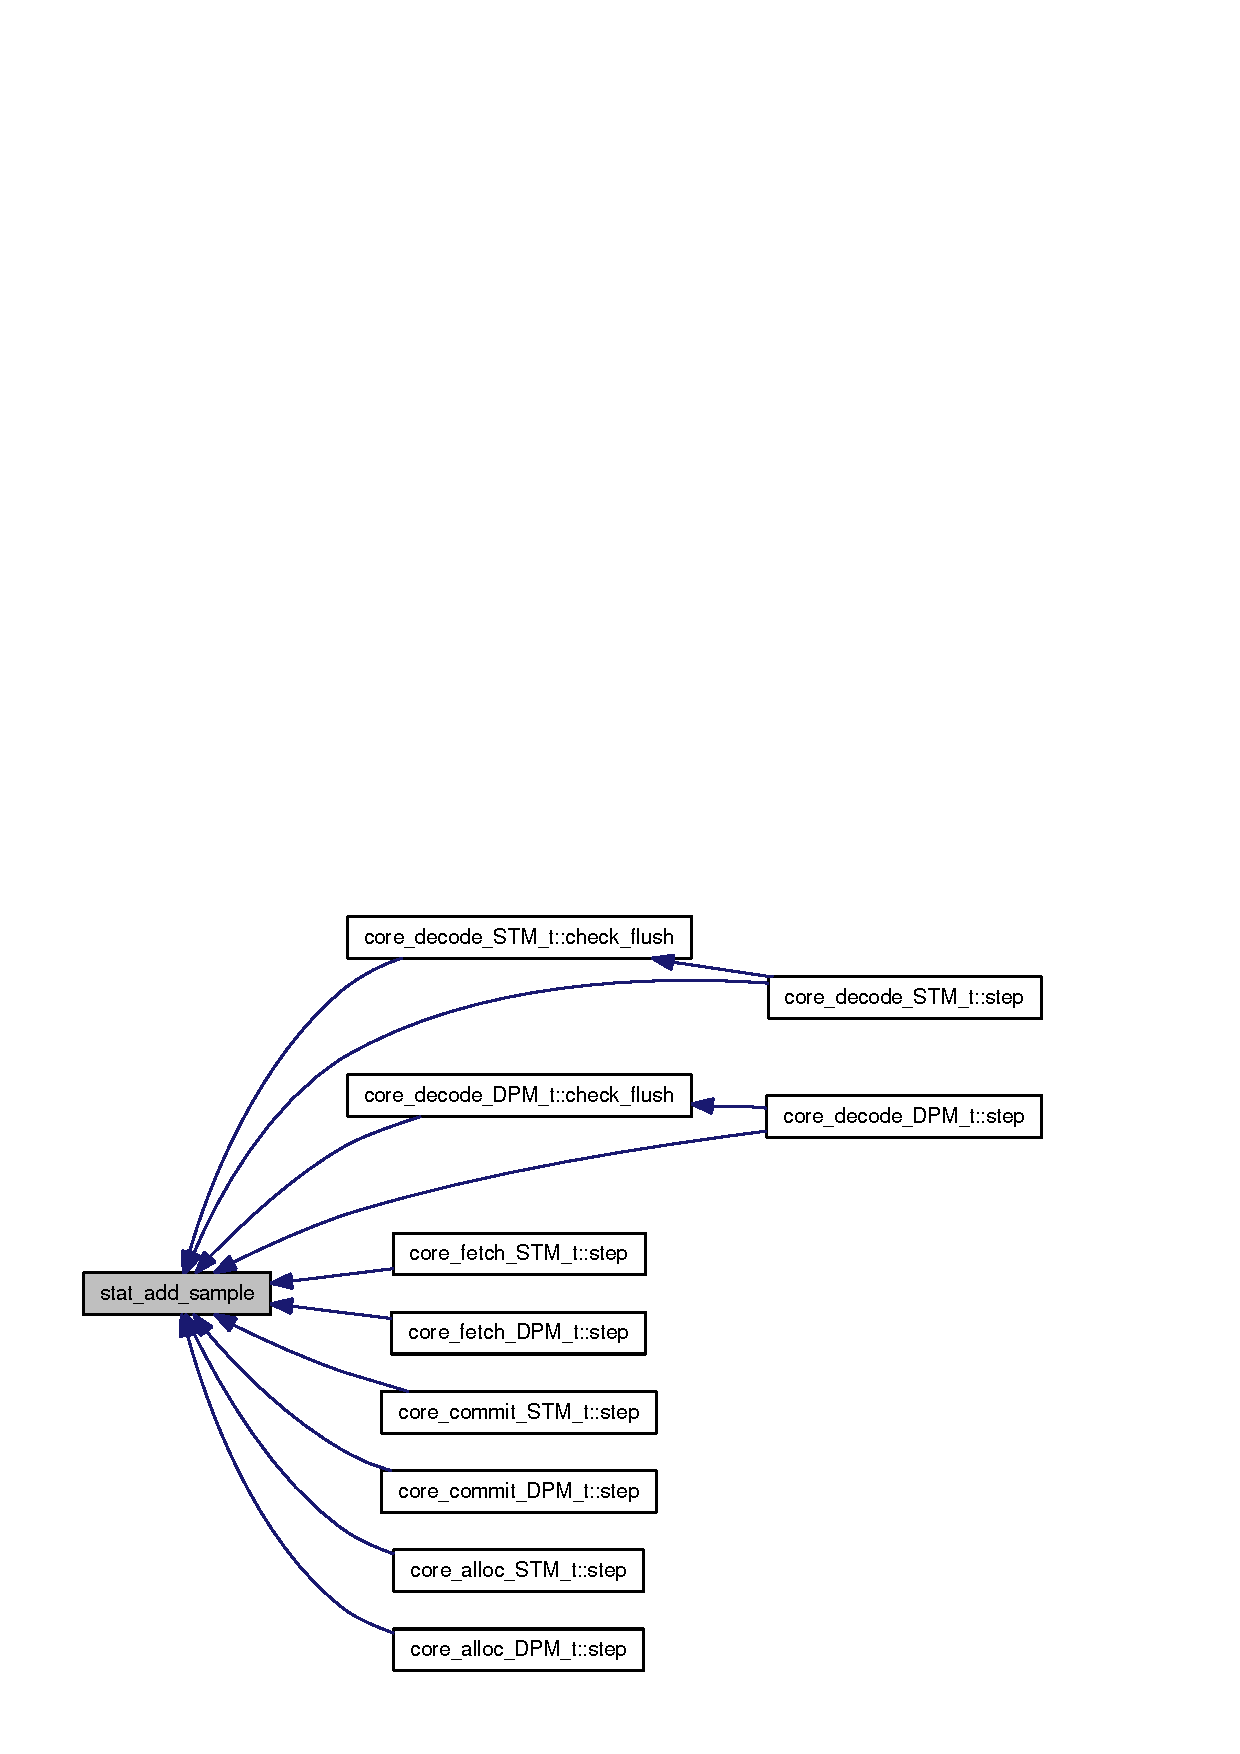
\includegraphics[width=252pt]{zesto_2stats_8h_702503b8068fdcce1dc8712be9791d42_icgraph}
\end{center}
\end{figure}
\index{zesto/stats.h@{zesto/stats.h}!stat\_\-add\_\-samples@{stat\_\-add\_\-samples}}
\index{stat\_\-add\_\-samples@{stat\_\-add\_\-samples}!zesto/stats.h@{zesto/stats.h}}
\subsubsection[{stat\_\-add\_\-samples}]{\setlength{\rightskip}{0pt plus 5cm}void stat\_\-add\_\-samples (struct {\bf stat\_\-stat\_\-t} $\ast$ {\em stat}, \/  {\bf md\_\-addr\_\-t} {\em index}, \/  int {\em nsamples})}\label{zesto_2stats_8h_d19289478f3e4e33e7b5a0caa68bd5b5}


\index{zesto/stats.h@{zesto/stats.h}!stat\_\-delete@{stat\_\-delete}}
\index{stat\_\-delete@{stat\_\-delete}!zesto/stats.h@{zesto/stats.h}}
\subsubsection[{stat\_\-delete}]{\setlength{\rightskip}{0pt plus 5cm}void stat\_\-delete (struct {\bf stat\_\-sdb\_\-t} $\ast$ {\em sdb})}\label{zesto_2stats_8h_c05227b0026bef4b301e9d8bdf3fcab7}


\index{zesto/stats.h@{zesto/stats.h}!stat\_\-eval\_\-ident@{stat\_\-eval\_\-ident}}
\index{stat\_\-eval\_\-ident@{stat\_\-eval\_\-ident}!zesto/stats.h@{zesto/stats.h}}
\subsubsection[{stat\_\-eval\_\-ident}]{\setlength{\rightskip}{0pt plus 5cm}struct {\bf eval\_\-value\_\-t} stat\_\-eval\_\-ident (struct {\bf eval\_\-state\_\-t} $\ast$ {\em es})\hspace{0.3cm}{\tt  [read]}}\label{zesto_2stats_8h_d675ee9049262ae066d7624c9c60f7e7}


\index{zesto/stats.h@{zesto/stats.h}!stat\_\-find\_\-stat@{stat\_\-find\_\-stat}}
\index{stat\_\-find\_\-stat@{stat\_\-find\_\-stat}!zesto/stats.h@{zesto/stats.h}}
\subsubsection[{stat\_\-find\_\-stat}]{\setlength{\rightskip}{0pt plus 5cm}struct {\bf stat\_\-stat\_\-t}$\ast$ stat\_\-find\_\-stat (struct {\bf stat\_\-sdb\_\-t} $\ast$ {\em sdb}, \/  const char $\ast$ {\em stat\_\-name})\hspace{0.3cm}{\tt  [read]}}\label{zesto_2stats_8h_e194205b24efd7c8a7c383156edce994}


\index{zesto/stats.h@{zesto/stats.h}!stat\_\-new@{stat\_\-new}}
\index{stat\_\-new@{stat\_\-new}!zesto/stats.h@{zesto/stats.h}}
\subsubsection[{stat\_\-new}]{\setlength{\rightskip}{0pt plus 5cm}struct {\bf stat\_\-sdb\_\-t}$\ast$ stat\_\-new (void)\hspace{0.3cm}{\tt  [read]}}\label{zesto_2stats_8h_cf6221385da9c71331ab5e4f718299da}




Referenced by main().

Here is the caller graph for this function:\nopagebreak
\begin{figure}[H]
\begin{center}
\leavevmode
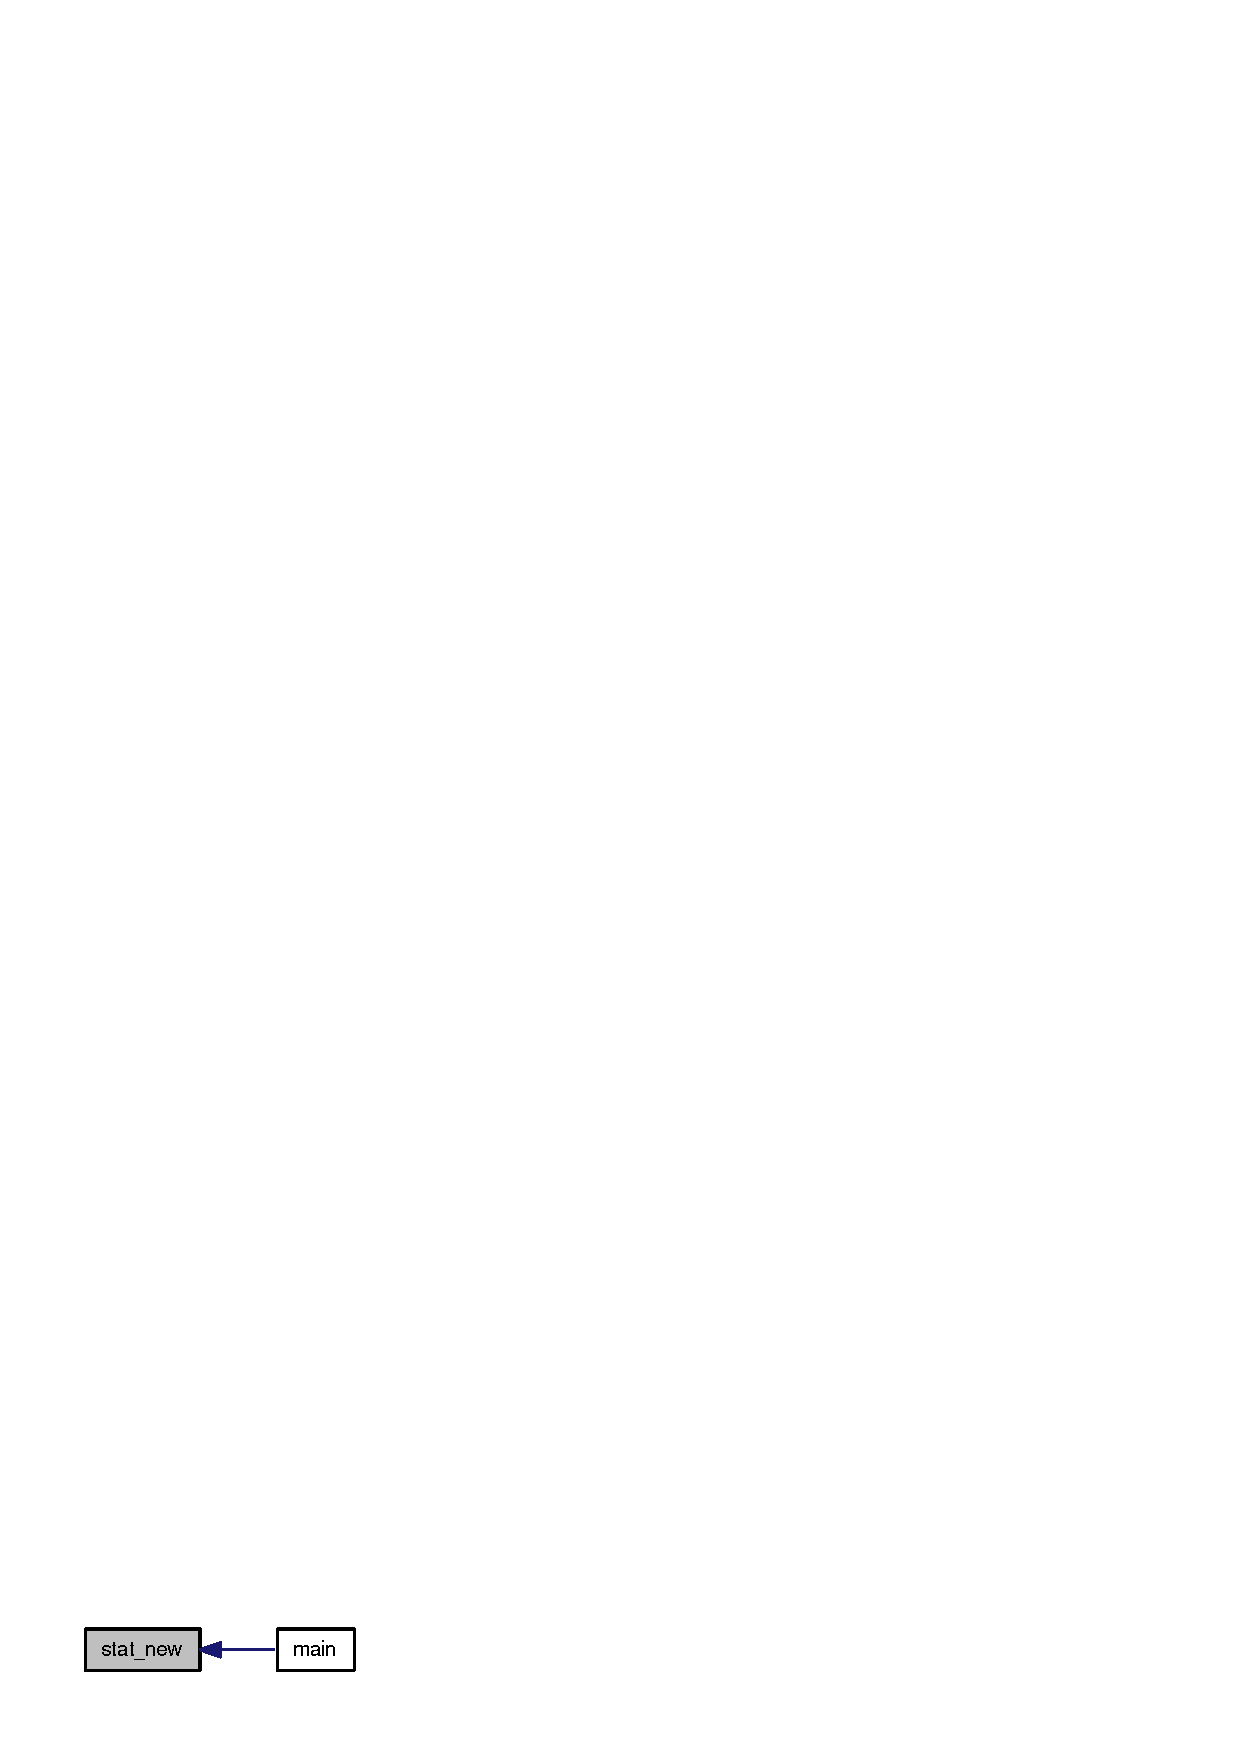
\includegraphics[width=87pt]{zesto_2stats_8h_cf6221385da9c71331ab5e4f718299da_icgraph}
\end{center}
\end{figure}
\index{zesto/stats.h@{zesto/stats.h}!stat\_\-print\_\-stat@{stat\_\-print\_\-stat}}
\index{stat\_\-print\_\-stat@{stat\_\-print\_\-stat}!zesto/stats.h@{zesto/stats.h}}
\subsubsection[{stat\_\-print\_\-stat}]{\setlength{\rightskip}{0pt plus 5cm}void stat\_\-print\_\-stat (struct {\bf stat\_\-sdb\_\-t} $\ast$ {\em sdb}, \/  struct {\bf stat\_\-stat\_\-t} $\ast$ {\em stat}, \/  FILE $\ast$ {\em fd})}\label{zesto_2stats_8h_1e642b17270bf002137ad70b5438b77c}


\index{zesto/stats.h@{zesto/stats.h}!stat\_\-print\_\-stats@{stat\_\-print\_\-stats}}
\index{stat\_\-print\_\-stats@{stat\_\-print\_\-stats}!zesto/stats.h@{zesto/stats.h}}
\subsubsection[{stat\_\-print\_\-stats}]{\setlength{\rightskip}{0pt plus 5cm}void stat\_\-print\_\-stats (struct {\bf stat\_\-sdb\_\-t} $\ast$ {\em sdb}, \/  FILE $\ast$ {\em fd})}\label{zesto_2stats_8h_dd36287ed8d81f546fb36bae677fb531}


\index{zesto/stats.h@{zesto/stats.h}!stat\_\-reg\_\-dist@{stat\_\-reg\_\-dist}}
\index{stat\_\-reg\_\-dist@{stat\_\-reg\_\-dist}!zesto/stats.h@{zesto/stats.h}}
\subsubsection[{stat\_\-reg\_\-dist}]{\setlength{\rightskip}{0pt plus 5cm}struct {\bf stat\_\-stat\_\-t}$\ast$ stat\_\-reg\_\-dist (struct {\bf stat\_\-sdb\_\-t} $\ast$ {\em sdb}, \/  const char $\ast$ {\em name}, \/  const char $\ast$ {\em desc}, \/  unsigned int {\em init\_\-val}, \/  unsigned int {\em arr\_\-sz}, \/  unsigned int {\em bucket\_\-sz}, \/  int {\em pf}, \/  const char $\ast$ {\em format}, \/  const char $\ast$$\ast$ {\em imap}, \/  {\bf print\_\-fn\_\-t} {\em print\_\-fn})\hspace{0.3cm}{\tt  [read]}}\label{zesto_2stats_8h_b68118a778041ff66b7dec8bf1030ef4}




Referenced by core\_\-fetch\_\-STM\_\-t::reg\_\-stats(), core\_\-fetch\_\-DPM\_\-t::reg\_\-stats(), core\_\-decode\_\-STM\_\-t::reg\_\-stats(), core\_\-decode\_\-DPM\_\-t::reg\_\-stats(), core\_\-commit\_\-STM\_\-t::reg\_\-stats(), core\_\-commit\_\-DPM\_\-t::reg\_\-stats(), core\_\-alloc\_\-STM\_\-t::reg\_\-stats(), and core\_\-alloc\_\-DPM\_\-t::reg\_\-stats().

Here is the caller graph for this function:\nopagebreak
\begin{figure}[H]
\begin{center}
\leavevmode
\includegraphics[width=153pt]{zesto_2stats_8h_b68118a778041ff66b7dec8bf1030ef4_icgraph}
\end{center}
\end{figure}
\index{zesto/stats.h@{zesto/stats.h}!stat\_\-reg\_\-double@{stat\_\-reg\_\-double}}
\index{stat\_\-reg\_\-double@{stat\_\-reg\_\-double}!zesto/stats.h@{zesto/stats.h}}
\subsubsection[{stat\_\-reg\_\-double}]{\setlength{\rightskip}{0pt plus 5cm}struct {\bf stat\_\-stat\_\-t}$\ast$ stat\_\-reg\_\-double (struct {\bf stat\_\-sdb\_\-t} $\ast$ {\em sdb}, \/  int {\em print\_\-me}, \/  const char $\ast$ {\em name}, \/  const char $\ast$ {\em desc}, \/  double $\ast$ {\em var}, \/  double {\em init\_\-val}, \/  const char $\ast$ {\em format})\hspace{0.3cm}{\tt  [read]}}\label{zesto_2stats_8h_be1b2059ba7cd215a0dddb2da620dbaf}


\index{zesto/stats.h@{zesto/stats.h}!stat\_\-reg\_\-float@{stat\_\-reg\_\-float}}
\index{stat\_\-reg\_\-float@{stat\_\-reg\_\-float}!zesto/stats.h@{zesto/stats.h}}
\subsubsection[{stat\_\-reg\_\-float}]{\setlength{\rightskip}{0pt plus 5cm}struct {\bf stat\_\-stat\_\-t}$\ast$ stat\_\-reg\_\-float (struct {\bf stat\_\-sdb\_\-t} $\ast$ {\em sdb}, \/  int {\em print\_\-me}, \/  const char $\ast$ {\em name}, \/  const char $\ast$ {\em desc}, \/  float $\ast$ {\em var}, \/  float {\em init\_\-val}, \/  const char $\ast$ {\em format})\hspace{0.3cm}{\tt  [read]}}\label{zesto_2stats_8h_378cfba0435cd73f9c4ecb78c2d64681}


\index{zesto/stats.h@{zesto/stats.h}!stat\_\-reg\_\-formula@{stat\_\-reg\_\-formula}}
\index{stat\_\-reg\_\-formula@{stat\_\-reg\_\-formula}!zesto/stats.h@{zesto/stats.h}}
\subsubsection[{stat\_\-reg\_\-formula}]{\setlength{\rightskip}{0pt plus 5cm}struct {\bf stat\_\-stat\_\-t}$\ast$ stat\_\-reg\_\-formula (struct {\bf stat\_\-sdb\_\-t} $\ast$ {\em sdb}, \/  int {\em print\_\-me}, \/  const char $\ast$ {\em name}, \/  const char $\ast$ {\em desc}, \/  const char $\ast$ {\em formula}, \/  const char $\ast$ {\em format})\hspace{0.3cm}{\tt  [read]}}\label{zesto_2stats_8h_f2f491659903b1b21de69fe6c767a64a}




Referenced by bus\_\-reg\_\-stats(), cache\_\-reg\_\-stats(), LLC\_\-reg\_\-stats(), prefetch\_\-t::reg\_\-stats(), core\_\-oracle\_\-t::reg\_\-stats(), memdep\_\-t::reg\_\-stats(), MC\_\-t::reg\_\-stats(), dram\_\-t::reg\_\-stats(), bpred\_\-t::reg\_\-stats(), RAS\_\-t::reg\_\-stats(), BTB\_\-t::reg\_\-stats(), fusion\_\-t::reg\_\-stats(), bpred\_\-dir\_\-t::reg\_\-stats(), core\_\-fetch\_\-STM\_\-t::reg\_\-stats(), core\_\-fetch\_\-DPM\_\-t::reg\_\-stats(), core\_\-exec\_\-STM\_\-t::reg\_\-stats(), core\_\-exec\_\-DPM\_\-t::reg\_\-stats(), core\_\-decode\_\-STM\_\-t::reg\_\-stats(), core\_\-decode\_\-DPM\_\-t::reg\_\-stats(), core\_\-commit\_\-STM\_\-t::reg\_\-stats(), core\_\-commit\_\-DPM\_\-t::reg\_\-stats(), core\_\-alloc\_\-STM\_\-t::reg\_\-stats(), core\_\-alloc\_\-DPM\_\-t::reg\_\-stats(), and uncore\_\-t::uncore\_\-reg\_\-stats().

Here is the caller graph for this function:\nopagebreak
\begin{figure}[H]
\begin{center}
\leavevmode
\includegraphics[width=338pt]{zesto_2stats_8h_f2f491659903b1b21de69fe6c767a64a_icgraph}
\end{center}
\end{figure}
\index{zesto/stats.h@{zesto/stats.h}!stat\_\-reg\_\-int@{stat\_\-reg\_\-int}}
\index{stat\_\-reg\_\-int@{stat\_\-reg\_\-int}!zesto/stats.h@{zesto/stats.h}}
\subsubsection[{stat\_\-reg\_\-int}]{\setlength{\rightskip}{0pt plus 5cm}struct {\bf stat\_\-stat\_\-t}$\ast$ stat\_\-reg\_\-int (struct {\bf stat\_\-sdb\_\-t} $\ast$ {\em sdb}, \/  int {\em print\_\-me}, \/  const char $\ast$ {\em name}, \/  const char $\ast$ {\em desc}, \/  int $\ast$ {\em var}, \/  int {\em init\_\-val}, \/  const char $\ast$ {\em format})\hspace{0.3cm}{\tt  [read]}}\label{zesto_2stats_8h_29b54a586f4845a6bb5dabbe04ad43be}




Referenced by prefetch\_\-t::reg\_\-stats(), memdep\_\-t::reg\_\-stats(), dram\_\-t::reg\_\-stats(), RAS\_\-t::reg\_\-stats(), BTB\_\-t::reg\_\-stats(), fusion\_\-t::reg\_\-stats(), and bpred\_\-dir\_\-t::reg\_\-stats().

Here is the caller graph for this function:\nopagebreak
\begin{figure}[H]
\begin{center}
\leavevmode
\includegraphics[width=292pt]{zesto_2stats_8h_29b54a586f4845a6bb5dabbe04ad43be_icgraph}
\end{center}
\end{figure}
\index{zesto/stats.h@{zesto/stats.h}!stat\_\-reg\_\-note@{stat\_\-reg\_\-note}}
\index{stat\_\-reg\_\-note@{stat\_\-reg\_\-note}!zesto/stats.h@{zesto/stats.h}}
\subsubsection[{stat\_\-reg\_\-note}]{\setlength{\rightskip}{0pt plus 5cm}struct {\bf stat\_\-stat\_\-t}$\ast$ stat\_\-reg\_\-note (struct {\bf stat\_\-sdb\_\-t} $\ast$ {\em sdb}, \/  const char $\ast$ {\em note})\hspace{0.3cm}{\tt  [read]}}\label{zesto_2stats_8h_ed9b9c4535e4fc2e59a090d6e8157d4f}




Referenced by core\_\-oracle\_\-t::reg\_\-stats(), core\_\-fetch\_\-STM\_\-t::reg\_\-stats(), core\_\-fetch\_\-DPM\_\-t::reg\_\-stats(), core\_\-exec\_\-STM\_\-t::reg\_\-stats(), core\_\-exec\_\-DPM\_\-t::reg\_\-stats(), core\_\-decode\_\-STM\_\-t::reg\_\-stats(), core\_\-decode\_\-DPM\_\-t::reg\_\-stats(), core\_\-commit\_\-STM\_\-t::reg\_\-stats(), core\_\-commit\_\-DPM\_\-t::reg\_\-stats(), core\_\-alloc\_\-STM\_\-t::reg\_\-stats(), core\_\-alloc\_\-DPM\_\-t::reg\_\-stats(), and uncore\_\-t::uncore\_\-reg\_\-stats().

Here is the caller graph for this function:\nopagebreak
\begin{figure}[H]
\begin{center}
\leavevmode
\includegraphics[width=155pt]{zesto_2stats_8h_ed9b9c4535e4fc2e59a090d6e8157d4f_icgraph}
\end{center}
\end{figure}
\index{zesto/stats.h@{zesto/stats.h}!stat\_\-reg\_\-qword@{stat\_\-reg\_\-qword}}
\index{stat\_\-reg\_\-qword@{stat\_\-reg\_\-qword}!zesto/stats.h@{zesto/stats.h}}
\subsubsection[{stat\_\-reg\_\-qword}]{\setlength{\rightskip}{0pt plus 5cm}struct {\bf stat\_\-stat\_\-t}$\ast$ stat\_\-reg\_\-qword (struct {\bf stat\_\-sdb\_\-t} $\ast$ {\em sdb}, \/  int {\em print\_\-me}, \/  const char $\ast$ {\em name}, \/  const char $\ast$ {\em desc}, \/  qword\_\-t $\ast$ {\em var}, \/  qword\_\-t {\em init\_\-val}, \/  const char $\ast$ {\em format})\hspace{0.3cm}{\tt  [read]}}\label{zesto_2stats_8h_d3b207566a223483451c345114249ac6}




Referenced by core\_\-commit\_\-STM\_\-t::reg\_\-stats(), and core\_\-commit\_\-DPM\_\-t::reg\_\-stats().

Here is the caller graph for this function:\nopagebreak
\begin{figure}[H]
\begin{center}
\leavevmode
\includegraphics[width=158pt]{zesto_2stats_8h_d3b207566a223483451c345114249ac6_icgraph}
\end{center}
\end{figure}
\index{zesto/stats.h@{zesto/stats.h}!stat\_\-reg\_\-sdist@{stat\_\-reg\_\-sdist}}
\index{stat\_\-reg\_\-sdist@{stat\_\-reg\_\-sdist}!zesto/stats.h@{zesto/stats.h}}
\subsubsection[{stat\_\-reg\_\-sdist}]{\setlength{\rightskip}{0pt plus 5cm}struct {\bf stat\_\-stat\_\-t}$\ast$ stat\_\-reg\_\-sdist (struct {\bf stat\_\-sdb\_\-t} $\ast$ {\em sdb}, \/  const char $\ast$ {\em name}, \/  const char $\ast$ {\em desc}, \/  unsigned int {\em init\_\-val}, \/  int {\em pf}, \/  const char $\ast$ {\em format}, \/  {\bf print\_\-fn\_\-t} {\em print\_\-fn})\hspace{0.3cm}{\tt  [read]}}\label{zesto_2stats_8h_ac098a3587e13dc2a0767f54d46e98c5}


\index{zesto/stats.h@{zesto/stats.h}!stat\_\-reg\_\-sqword@{stat\_\-reg\_\-sqword}}
\index{stat\_\-reg\_\-sqword@{stat\_\-reg\_\-sqword}!zesto/stats.h@{zesto/stats.h}}
\subsubsection[{stat\_\-reg\_\-sqword}]{\setlength{\rightskip}{0pt plus 5cm}struct {\bf stat\_\-stat\_\-t}$\ast$ stat\_\-reg\_\-sqword (struct {\bf stat\_\-sdb\_\-t} $\ast$ {\em sdb}, \/  int {\em print\_\-me}, \/  const char $\ast$ {\em name}, \/  const char $\ast$ {\em desc}, \/  sqword\_\-t $\ast$ {\em var}, \/  sqword\_\-t {\em init\_\-val}, \/  const char $\ast$ {\em format})\hspace{0.3cm}{\tt  [read]}}\label{zesto_2stats_8h_6c7a4257d59d1a3f3d8056326d3ab3ba}


\index{zesto/stats.h@{zesto/stats.h}!stat\_\-reg\_\-string@{stat\_\-reg\_\-string}}
\index{stat\_\-reg\_\-string@{stat\_\-reg\_\-string}!zesto/stats.h@{zesto/stats.h}}
\subsubsection[{stat\_\-reg\_\-string}]{\setlength{\rightskip}{0pt plus 5cm}struct {\bf stat\_\-stat\_\-t}$\ast$ stat\_\-reg\_\-string (struct {\bf stat\_\-sdb\_\-t} $\ast$ {\em sdb}, \/  const char $\ast$ {\em name}, \/  const char $\ast$ {\em desc}, \/  const char $\ast$ {\em var}, \/  const char $\ast$ {\em format})\hspace{0.3cm}{\tt  [read]}}\label{zesto_2stats_8h_c8c6f5229297787dbce204434f45acce}




Referenced by memdep\_\-t::reg\_\-stats(), RAS\_\-t::reg\_\-stats(), BTB\_\-t::reg\_\-stats(), fusion\_\-t::reg\_\-stats(), and bpred\_\-dir\_\-t::reg\_\-stats().

Here is the caller graph for this function:\nopagebreak
\begin{figure}[H]
\begin{center}
\leavevmode
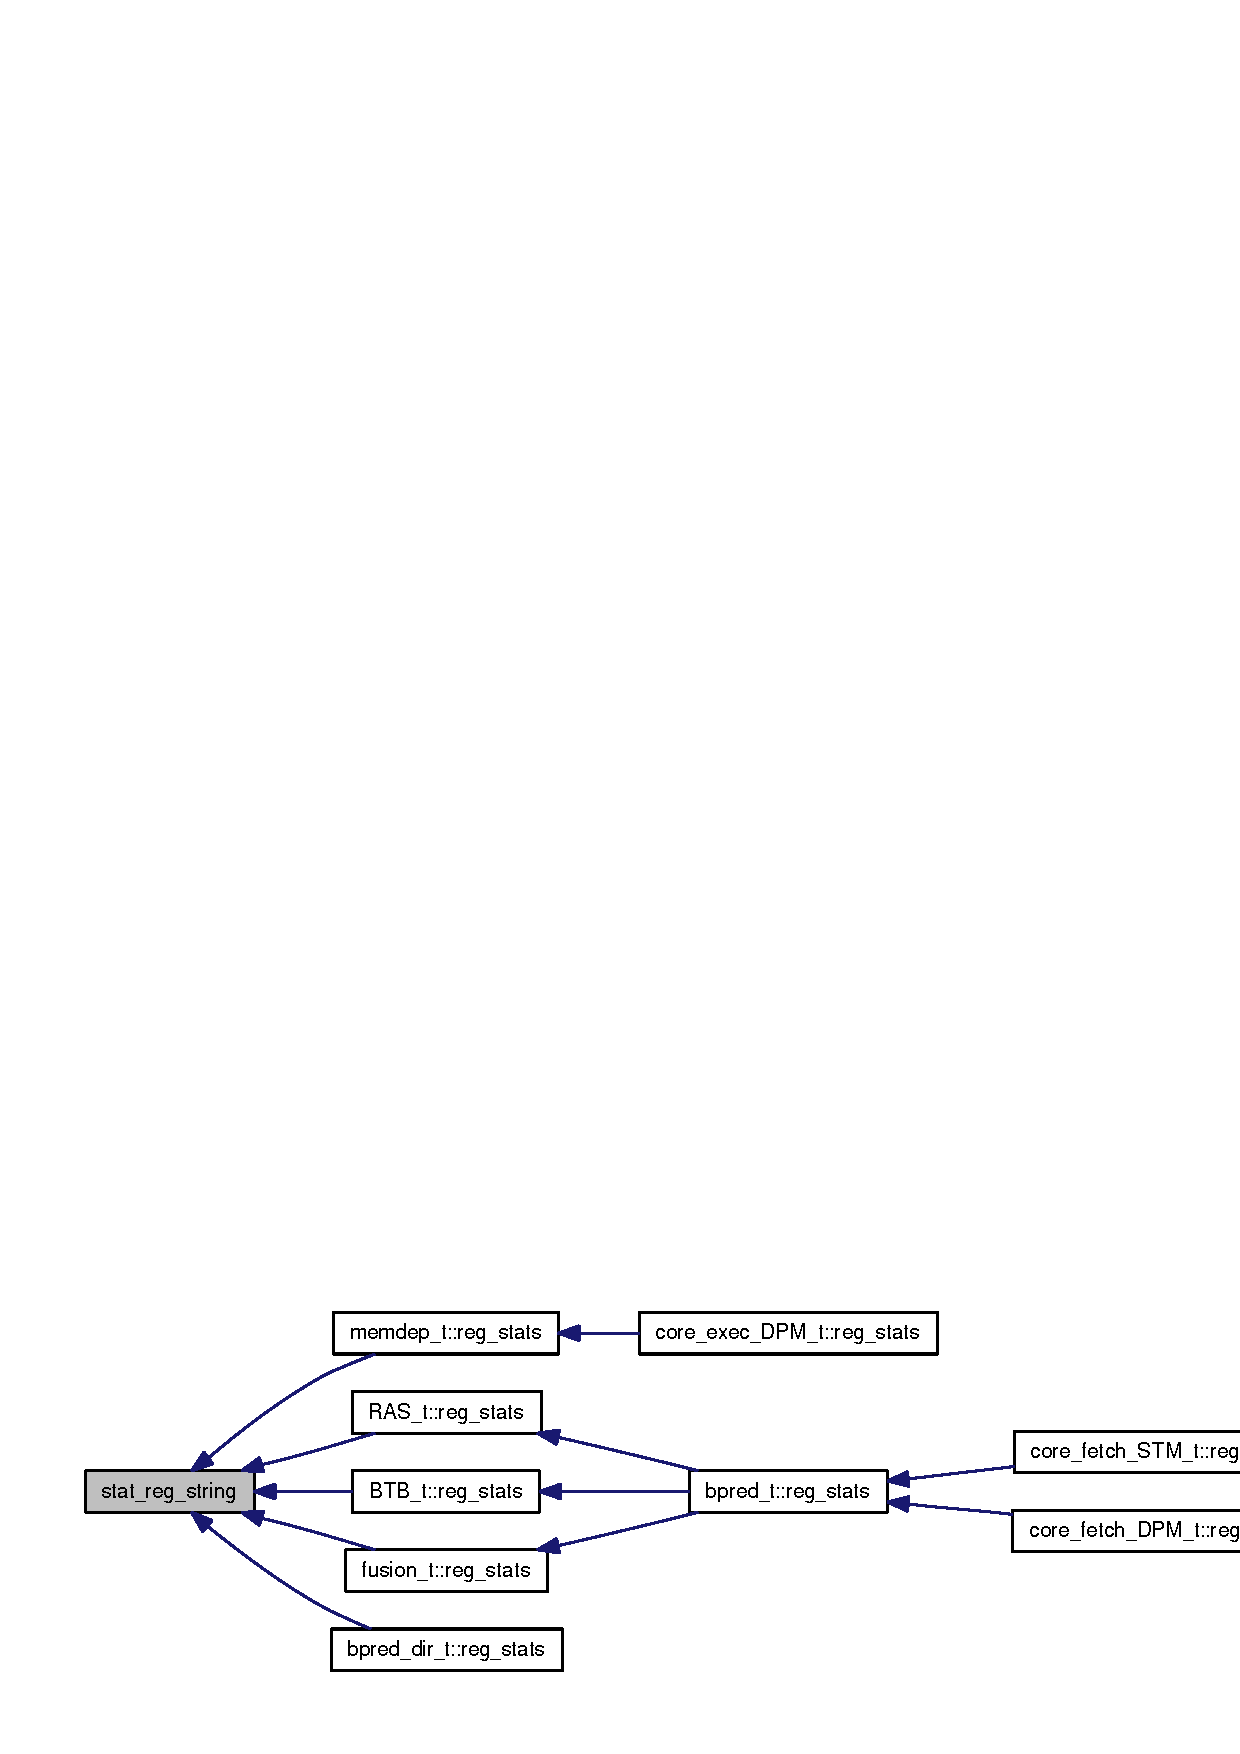
\includegraphics[width=317pt]{zesto_2stats_8h_c8c6f5229297787dbce204434f45acce_icgraph}
\end{center}
\end{figure}
\index{zesto/stats.h@{zesto/stats.h}!stat\_\-reg\_\-uint@{stat\_\-reg\_\-uint}}
\index{stat\_\-reg\_\-uint@{stat\_\-reg\_\-uint}!zesto/stats.h@{zesto/stats.h}}
\subsubsection[{stat\_\-reg\_\-uint}]{\setlength{\rightskip}{0pt plus 5cm}struct {\bf stat\_\-stat\_\-t}$\ast$ stat\_\-reg\_\-uint (struct {\bf stat\_\-sdb\_\-t} $\ast$ {\em sdb}, \/  int {\em print\_\-me}, \/  const char $\ast$ {\em name}, \/  const char $\ast$ {\em desc}, \/  unsigned int $\ast$ {\em var}, \/  unsigned int {\em init\_\-val}, \/  const char $\ast$ {\em format})\hspace{0.3cm}{\tt  [read]}}\label{zesto_2stats_8h_bc60b66d6bc63111e715425410f1156a}


